\section{Experimentación}

\todo[inline]{Experimentacion general pensar mas:  }
\todo[inline]{Diferencias de tiempos EG vs LU, con si y mascara mascara}
\todo[inline]{Mostrar como con diferentes luces obtenemos diferentes normales}
\todo[inline]{Mostrar resultados finales con mismas luces pero propias vs catedra}


% 1. Comparar las direcciones de iluminacion obtenidas por el metodo de calibracion con las provistas por la catedra \\

Veamos qué tan buena fue nuestra calibración. Dado que la cátedra nos brindó los vectores de luces lo que nos gustaría hacer es comparar ambos. En general, niguna luz quedó \textit{exactamente} igual, pero sí quedaron similares. \\

Dado que es complicado visulizar diferencias entre vectores tridimensionales, analizaremos por un lado el eje $z$ y por el otro los ejes $x$ e $y$. En el siguiente gráfico tomamos para cada luz, los ejes $z$ y calculamos su diferencia. \\

{\centering
    \includegraphics[scale=0.7]{informe/imagenes/lucesEjezDiferencias.pdf} \\
}

Podemos observar que la la diferencia máxima es aproximadamente $0.1$ mientras que la diferencia mínima está cercana a cero (es exactamente $0.001821$ en la luz $1$). Creemos que si bien no es perfecto, es una diferencia aceptable. Dado que todos los vectores son unitarios (pues fueron normalizados) es lógico esperar diferencias entre los ejes x e y. A continuación puede verse el gráfico resultante. Las luces que se corresponden con las propias y las de la cátedra están señaladas con el mismo color. \\

Podemos observar que si bien las diferencias son notorias, todas se encuentran en el mismo rango en inclinación. No hay ninguna que haga cosas extrañas como apuntar en sentido inverso. Creemos que las diferencias no afectarán demasiado el resultado final.

{\centering
    \includegraphics[scale=0.8]{informe/imagenes/lucesCatedraProyeccionXY.pdf} \\
    % \captionof{figure}{Luces de la cátedra en la proyección x,y}
}
{\centering
    \includegraphics[scale=0.8]{informe/imagenes/lucesPropiasProyeccionXY.pdf} \\
    % \captionof{figure}{Luces propias en la proyección x,y}
}

$ $\newline

% 2. Como afecta la calibracion del sistema en el resto de las etapas \\

Dado que las luces son utilizadas para el cálculo de las normales, queremos ver cómo nos afecta la calibración en esta etapa. Para eso, resolveremos el sistema de ecuaciones y guardaremos los vectores normales obtenidos. Como las mayores diferencias entre luces podían verse en los ejes $x, y$ estos ejes serán los que usaremos en la comparación.

En los gráficos que se encuentran a continuación, para cada píxel se grafica un vector que corresponde a la normal en ese punto. Como son \textit{miles} de normales, puede dar la impresión de que se grafican puntos pero no es así: son los vectores en forma de 'flechas'. \\

$ $\newline

En todos los gráficos se utiliza exactamente la misma área de la imagen para que sean comparables. Para la resolución del sistema que calcula las normales se ultiliza eliminación gaussiana con pivoteo parcial para tratar de minimizar el error numérico. \\

Para nuestro primer experimento tomaremos nuestra 'mejor luz', la $1$ junto con las luces $4$ y $5$ que parecen ser las 'peores'. Los resultados fueron bastante buenos. \\

Las diferencias mas notorias se encuentran en el ojo y en la oreja del caballo. Creemos que tiene que ver porque son las áreas con más detalle pero menor iluminación. Sin embargo, no creemos que sea una diferencia demasiado significativa.

{\centering
    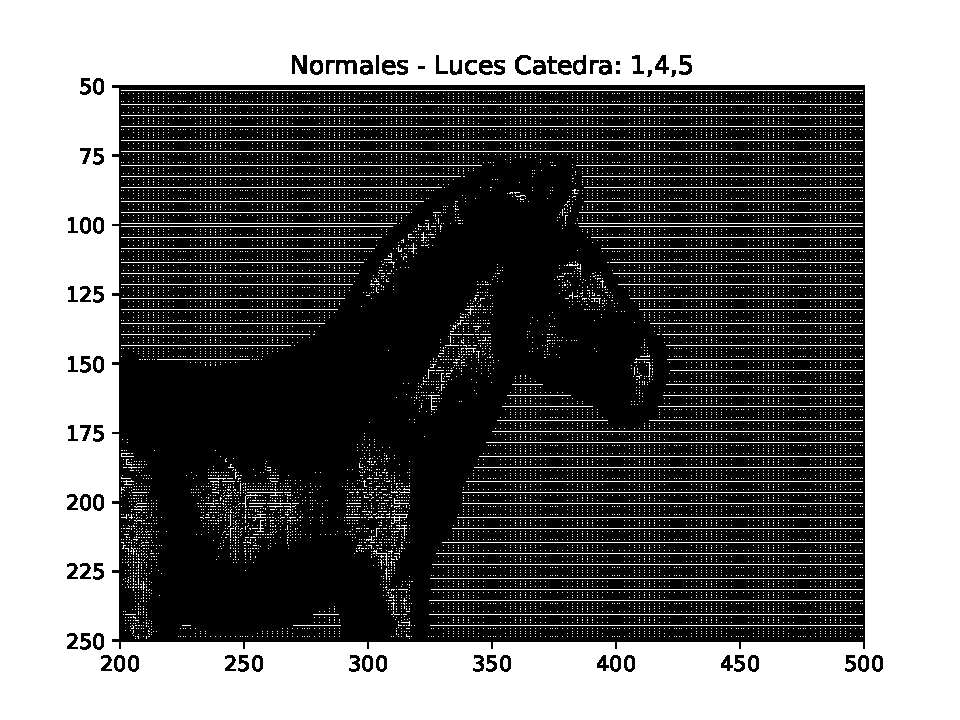
\includegraphics[scale=0.8]{informe/imagenes/normales/normalesCaballoLucesCatedra145.pdf} \\
}
{\centering
    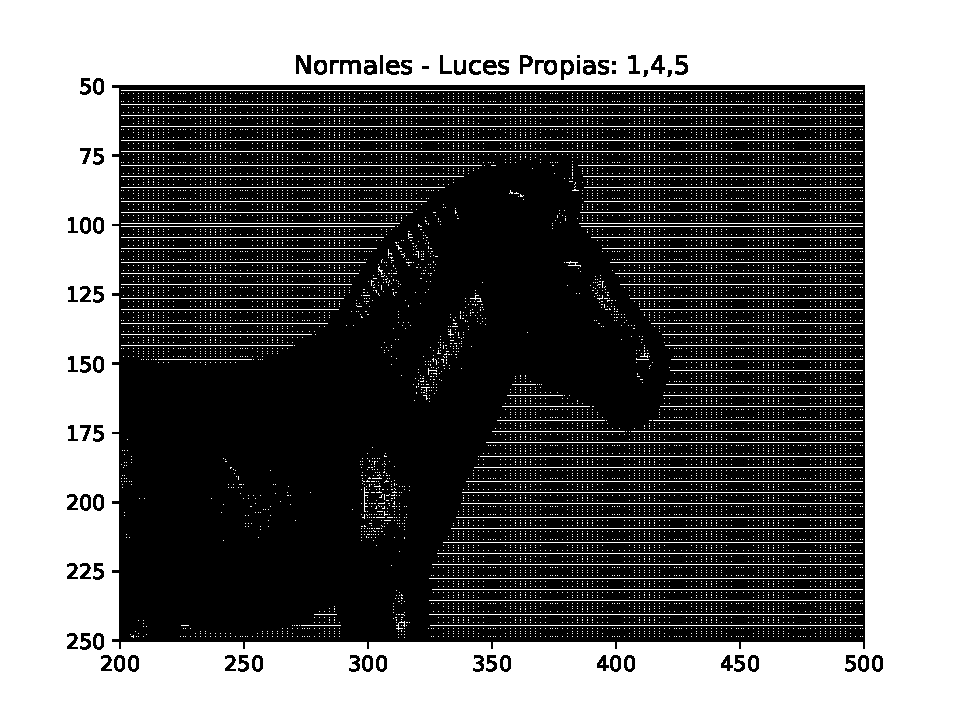
\includegraphics[scale=0.8]{informe/imagenes/normales/normalesCaballoLucesPropias145.pdf} \\
}

\newpage
Veamos que pasa si no tomamos la luz número $1$, que era la mejor que teníamos y en su lugar tomamos otra de las 'malas'. En este caso, consideraremos las luces $4,5$ y $6$. Tanto las de la cátedra como las propias son demasiado oscuras, sin embargo la nuestra lo es mucho más. Los rasgos faciales dejaron de apreciarse. \\

{\centering
    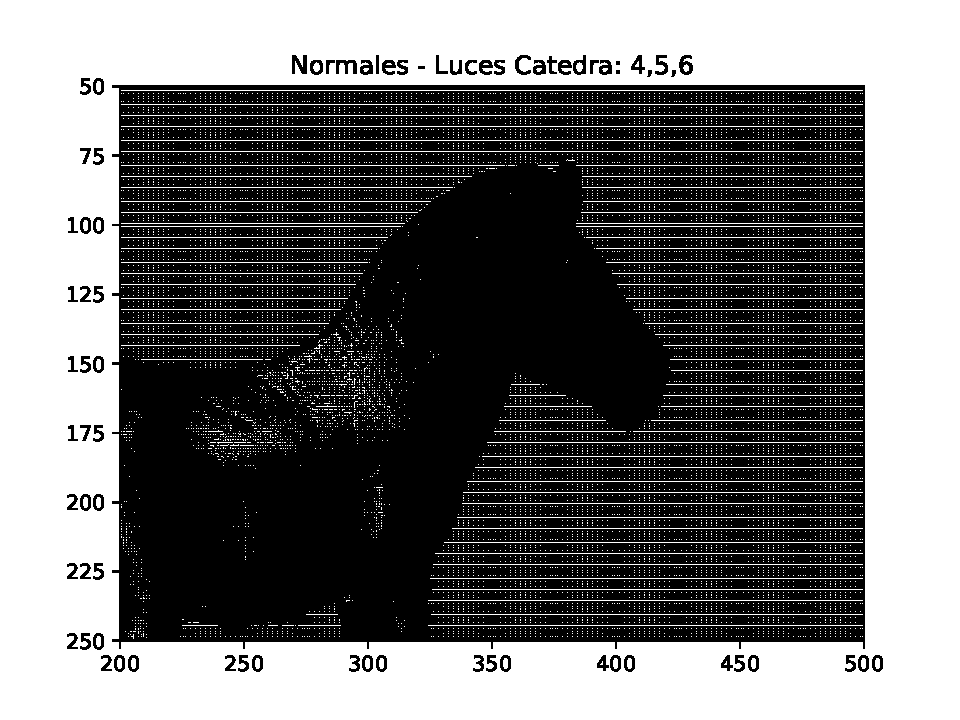
\includegraphics[scale=0.8]{informe/imagenes/normales/normalesCaballoLucesCatedra456.pdf} \\
}
{\centering
    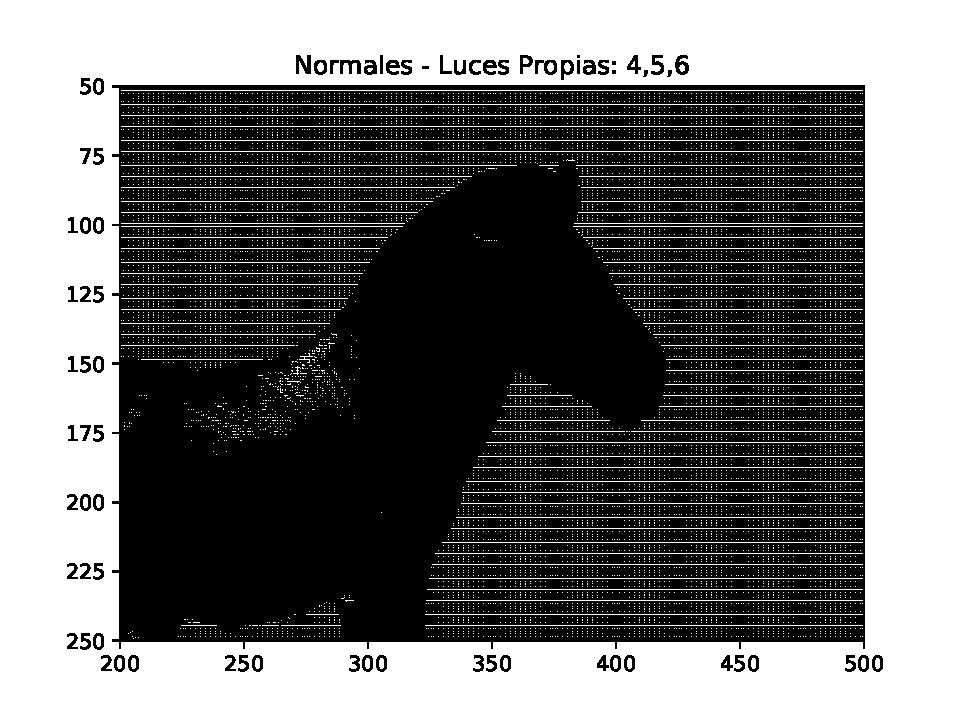
\includegraphics[scale=0.8]{informe/imagenes/normales/normalesCaballoLucesPropias456.pdf} \\
}

\newpage

Se pide por enunciado. \\
3. ¿Como impacta la eleccion de las 3 direcciones de iluminacion para el calculo de las normales? \\
